% Next-token prediction example diagram inspired by the provided reference
% Shows a single training example, target one-hot vector, and cross-entropy intuition

\documentclass{article}
\usepackage[margin=0.2cm, paperwidth=18.8cm, paperheight=8.4cm]{geometry}
\usepackage[T1]{fontenc}
\usepackage[scaled=0.95]{helvet}
\usepackage{sfmath}
\renewcommand{\familydefault}{\sfdefault}
\usepackage{tikz}
\usetikzlibrary{positioning, arrows.meta, calc, decorations.pathreplacing}
\pagestyle{empty}

\begin{document}

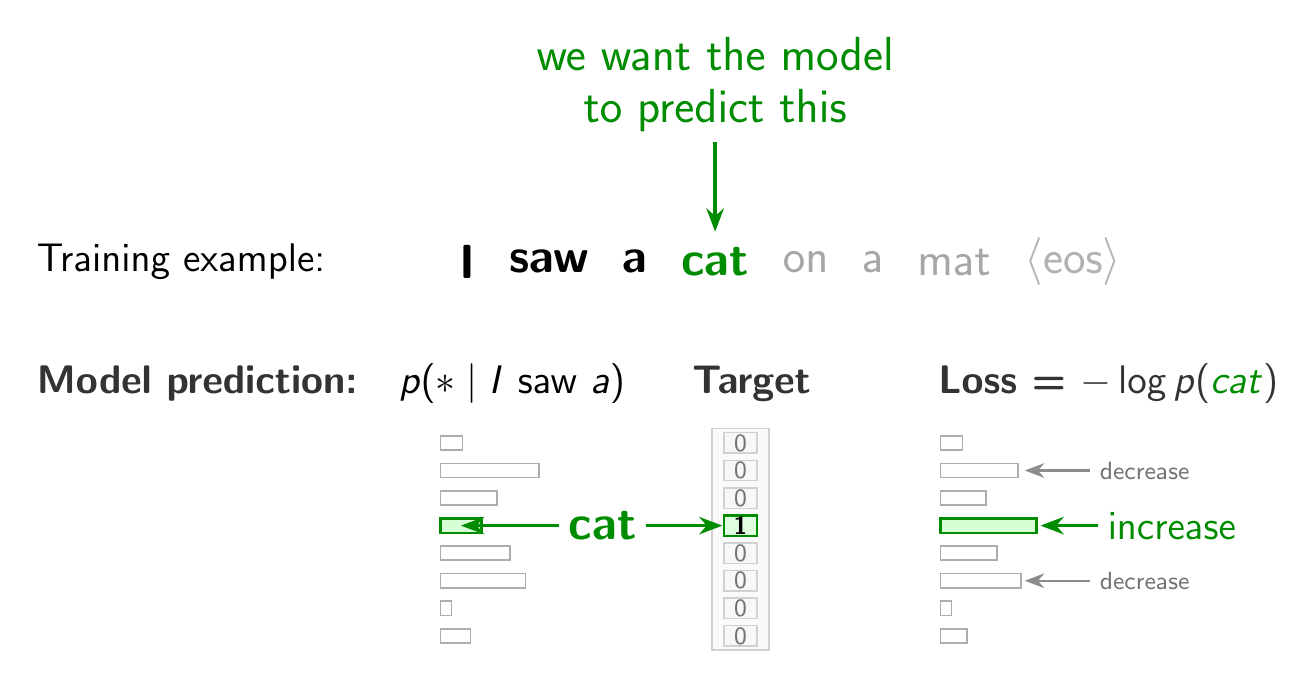
\begin{tikzpicture}[
    font=\sffamily,
    arrow/.style={->, >=Stealth, line width=1.0pt, draw=black!70},
    greenarrow/.style={->, >=Stealth, line width=1.2pt, draw=green!55!black},
    softarrow/.style={->, >=Stealth, line width=0.9pt, draw=black!45},
    note/.style={font=\small, text=black!55},
    section/.style={font=\bfseries\Large, text=black!80},
    bar/.style={draw=black!32, fill=white, line width=0.6pt},
    goodbar/.style={draw=green!55!black, fill=green!16, line width=0.8pt},
    targetbox/.style={draw=black!18, fill=black!3, line width=0.5pt},
    goodtarget/.style={draw=green!55!black, fill=green!12, line width=0.8pt}
]

% Training example sentence
\node[anchor=west, font=\Large] at (0.35, 5.25) {Training example:};
\node[anchor=west, font=\bfseries\fontsize{18}{20}\selectfont] (w1) at (5.72, 5.25) {I};
\node[anchor=west, font=\bfseries\fontsize{18}{20}\selectfont, right=0.18cm of w1] (w2) {saw};
\node[anchor=west, font=\bfseries\fontsize{18}{20}\selectfont, right=0.18cm of w2] (w3) {a};
\node[anchor=west, font=\bfseries\fontsize{18}{20}\selectfont, text=green!55!black, right=0.18cm of w3] (w4) {cat};
\node[anchor=west, font=\fontsize{18}{20}\selectfont, text=black!35, right=0.18cm of w4] (w5) {on};
\node[anchor=west, font=\fontsize{18}{20}\selectfont, text=black!35, right=0.18cm of w5] (w6) {a};
\node[anchor=west, font=\fontsize{18}{20}\selectfont, text=black!35, right=0.18cm of w6] (w7) {mat};
\node[anchor=west, font=\fontsize{18}{20}\selectfont, text=black!30, right=0.18cm of w7] (w8) {$\langle$eos$\rangle$};

% Top annotation
\node[align=center, text=green!55!black, font=\fontsize{17}{19}\selectfont] (topnote) at ($(w4.north)+(0,1.95)$)
    {we want the model\\to predict this};
\draw[greenarrow] (topnote.south) -- ($(w4.north)+(0,0.08)$);

% Section titles
\node[anchor=west, section] at (0.35, 3.7) {Model prediction:};
\node[anchor=west, font=\Large] at (4.95, 3.7) {$p(* \mid I\ \mathrm{saw}\ a)$};
\node[section] at (9.55, 3.7) {Target};
\node[anchor=west, section] at (11.8, 3.7) {Loss = $-\log p(\textcolor{green!55!black}{cat})$};

% Row positions
\def\yA{2.95}
\def\yB{2.60}
\def\yC{2.25}
\def\yD{1.90}
\def\yE{1.55}
\def\yF{1.20}
\def\yG{0.85}
\def\yH{0.50}
\def\predx{5.60}

% Left distribution bars
\draw[bar] (\predx,\yA-0.09) rectangle ++(0.28,0.18);
\draw[bar] (\predx,\yB-0.09) rectangle ++(1.25,0.18);
\draw[bar] (\predx,\yC-0.09) rectangle ++(0.72,0.18);
\draw[goodbar] (\predx,\yD-0.09) rectangle ++(0.52,0.18);
\draw[bar] (\predx,\yE-0.09) rectangle ++(0.88,0.18);
\draw[bar] (\predx,\yF-0.09) rectangle ++(1.08,0.18);
\draw[bar] (\predx,\yG-0.09) rectangle ++(0.14,0.18);
\draw[bar] (\predx,\yH-0.09) rectangle ++(0.38,0.18);

% Target vector
\draw[targetbox, fill=black!2] (9.05,\yH-0.18) rectangle (9.77,\yA+0.18);
\foreach \y/\val in {\yA/0,\yB/0,\yC/0,\yD/1,\yE/0,\yF/0,\yG/0,\yH/0} {
    \ifnum\val=1
        \draw[goodtarget] (9.2,\y-0.13) rectangle ++(0.42,0.26);
        \node[font=\bfseries\small] at (9.41,\y) {\val};
    \else
        \draw[targetbox] (9.2,\y-0.13) rectangle ++(0.42,0.26);
        \node[font=\small, text=black!55] at (9.41,\y) {\val};
    \fi
}

% Cat label and arrows
\node[text=green!55!black, font=\bfseries\fontsize{18}{20}\selectfont] (catlabel) at (7.66,\yD) {cat};
\draw[greenarrow] (catlabel.west) -- (\predx+0.26,\yD);
\draw[greenarrow] (catlabel.east) -- (9.18,\yD);

% Right distribution after minimizing loss
\draw[bar] (11.95,\yA-0.09) rectangle ++(0.28,0.18);
\draw[bar] (11.95,\yB-0.09) rectangle ++(0.98,0.18);
\draw[bar] (11.95,\yC-0.09) rectangle ++(0.58,0.18);
\draw[goodbar] (11.95,\yD-0.09) rectangle ++(1.22,0.18);
\draw[bar] (11.95,\yE-0.09) rectangle ++(0.72,0.18);
\draw[bar] (11.95,\yF-0.09) rectangle ++(1.02,0.18);
\draw[bar] (11.95,\yG-0.09) rectangle ++(0.14,0.18);
\draw[bar] (11.95,\yH-0.09) rectangle ++(0.34,0.18);

% Increase / decrease annotation
\node[anchor=west, note] (dectop) at (13.85, \yB) {decrease};
\draw[softarrow] (dectop.west) -- (13.02,\yB);
\node[anchor=west, text=green!55!black, font=\Large] (inc) at (13.95,\yD) {increase};
\draw[greenarrow] (inc.west) -- (13.22,\yD);
\node[anchor=west, note] (decbot) at (13.85, \yF) {decrease};
\draw[softarrow] (decbot.west) -- (13.02,\yF);

\end{tikzpicture}

\end{document}
